\section{System Architectures}

We implemented four architecture variations (\emph{Simple}, \emph{Simple-Crew}, \emph{Gateway}, and \emph{Gateway-RAG}). The first two follow conventional multi-agent coordination patterns, while the latter two represent a deliberate architectural departure by introducing our unified capability abstraction and gateway design. All four solve the same problem, which we define in the next section. However for now, we treat each architecture as task-agnostic and focus on interaction patterns.

\subsection{Simple Architectures}
\subsubsection{Simple Architecture}
\begin{figure}[ht]
    \centering
    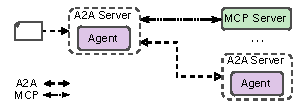
\includegraphics[width=\columnwidth]{figures/architectures/simple.pdf}
    \caption{Simple Architecture: Agents handle both MCP and A2A}
    \label{fig:simple}
\end{figure}

The simple architecture serves as our baseline and does not employ any optimizations for tool or agent retrieval. It can be viewed as the standard implementation path suggested by existing frameworks and protocols.

Each agent is exposed via the A2A protocol so that it can be invoked by other agents. A single agent receives an explicit configuration that determines its environment, namely which MCP servers it can interact with and which peer agents it can communicate with via A2A. All previously described information about tools and agents is loaded into the agent's context upon first connection to the respective MCP or A2A server. This means that all semantic and technical details for all tools and agents accumulate in the agent's context from the outset, and the agent bears the full responsibility of producing valid outputs that either its MCP or A2A client can parse.

This design leads to two compounding problems. First, the agent's context is populated with the full set of available tool descriptions and agent specifications, regardless of their relevance to the immediate planning task. This phenomenon is commonly referred to as \emph{context bloat}. Second, the agent must manage two distinct protocol conventions simultaneously, which increases the likelihood of \emph{protocol confusion}, where outputs become syntactically invalid for the intended client.\medskip

\subsubsection{Simple-Crew Architecture}
\begin{figure}[hb]
    \centering
    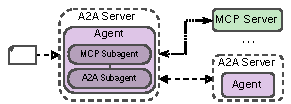
\includegraphics[width=\columnwidth]{figures/architectures/simple-crew.pdf}
    \caption{Simple-Crew Architecture: Agents are divided into crews of protocol-specific subagents}
    \label{fig:simple-crew}
\end{figure}
A natural first improvement is to split the responsibilities within an agent so that a given A2A-exposed agent is internally composed of two sub-agents: One dedicated to MCP tool retrieval and invocation, and another dedicated to communicating with peer agents via A2A.

This separation allows each sub-agent to specialize on a single protocol. 
Reducing the protocol confusion creates a new coordination overhead: The sub-agents must collaborate as a team, and each must understand at what stage it should take the lead, despite only having partial visibility into the full set of the agent's capabilities. While this problem is manageable when sub-agent tasks follow a known, relatively strict ordering, this implies that the architecture requires either careful manual specialization of the agent configuration or sufficiently capable sub-agents that can autonomously determine when to hand off control.

Crucially, the problem of context bloat remains unsolved in this architecture. Both sub-agents still receive the full tool descriptions or agent cards for their respective protocols. Instead the bloat is merely distributed across sub-agents that now additionally require coordination context about their partner.\medskip

\subsection{Simple Architecture Discussion}

Both simple architectures suffer from context bloat, and differ primarily in how they handle protocol confusion: The \emph{Simple} architecture exposes it fully to a single agent, while the \emph{Simple-Crew} variant trades it for coordination overhead. Moreover, both designs scale poorly as additional protocols emerge, since each new standard introduces further conventions and error semantics that agents must manage directly. These limitations motivate a fundamental shift away from direct protocol exposure toward a mediated interaction pattern, which we present next.

\subsection{Gateway Architectures}
\subsubsection{Gateway Architecture}
\begin{figure}[hb]
    \centering
    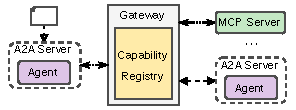
\includegraphics[width=\columnwidth]{figures/architectures/gateway.pdf}
    \caption{Gateway Architecture: Agents communicate through protocol-handling gateway with capability abstraction}
    \label{fig:gateway}
\end{figure}
The gateway architecture constitutes a central contribution of this paper and can be portrait as a refined proxy approach as introduced by the MCPBridge~\cite{ahmadi2026mcpbridge} or ToolRegistry~\cite{ding2025toolregistry}. In this variation, agents are no longer directly connected to MCP servers or peer agents via A2A. Instead, the gateway mediates all communication. It receives tool descriptions and agent cards from the underlying ecosystem and maps them into a unified capability data model, which constitutes a central abstraction of our system.\medskip

\paragraph*{Staged Information Exposure}
Both MCP tool descriptions and A2A Agent Cards intermingle natural-language descriptions of what a tool or agent can do with protocol-specific formats, authentication requirements, and other technical details. We argue that conflating these two categories of information is architecturally harmful. Agents benefit from reasoning about capability semantics during planning and selection, while protocol-level execution details should only enter the context once a capability has been selected and invocation is imminent. This principle, which we refer to as \emph{staged information exposure}, motivates a strict phasing of the information an agent receives. Rather than exposing all available metadata upfront, the gateway produces two representations for each capability: The \emph{capability summary}, which contains only semantic information about what a capability does, and the \emph{capability detail}, which additionally includes all technical specifics required for execution. As prior work has indicated, correct capability retrieval is essential for task success~\cite{mo2026livemcpbench}, and keeping the planning context free of irrelevant technical detail is designed to support exactly this.\medskip

The gateway exposes a deliberately thin API consisting of three endpoints that allow agents to: 
\begin{itemize}
\item Retrieve all capability summaries for the tools and agents available to them
\item Retrieve the full details of a specific capability given its unique identifier
\item Execute a specific capability with either a structured parameter dictionary or a plain-text handoff
\end{itemize}

Compared to MCPBridge~\cite{ahmadi2026mcpbridge} and ToolRegistry~\cite{ding2025toolregistry}, our gateway can handle tool invocation and agent communication protocols. Additionally our API is thiner and we support access both via a standard REST interface and via three lightweight MCP meta-tools. We intentionally designed the API to be as thin yet complete as possible, placing agents back into the regime that their underlying cognitive architectures were designed for. Most notably, ReAct~\cite{yao2023react} and similar frameworks assume reasoning over a very small tool set, and our design restores exactly this condition. 

This design fundamentally changes how agents interact with their environment. Instead of receiving all available tools and Agent Cards alongside the task input and system prompt at the start, the agent's context is initially kept deliberately small. The agent can therefore focus on understanding the concrete task requirements and its behavioral constraints first. Only after reasoning about this foundational information does the agent retrieve capability summaries and decide, based solely on semantic descriptions, which capabilities are best suited for each subtask and in which order to invoke them. As we will show later, this initial freedom and the semantic decision-making it enables, independent of protocol or technical details, helps achieving a substantially higher task success.\medskip

\subsubsection{Gateway-RAG Architecture}
\begin{figure}[ht]
    \centering
    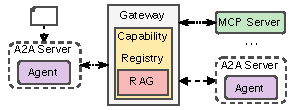
\includegraphics[width=\columnwidth]{figures/architectures/gateway-rag.pdf}
    \caption{Gateway-RAG Architecture: Gateway is extended with semantic capability retrieval}
    \label{fig:gateway-rag}
\end{figure}

Given the already competitive performance of the gateway architecture and inspired by the growing body of literature on semantic tool retrieval~\cite{gaurav2025dynamicreact, fei2025mcpzero, gan2025ragmcp, lumer2025scalemcp, lumer2025tooltoagent, gaurav2025codemem}, we implement a second gateway variation with a modified discovery mechanism. Instead of allowing agents to retrieve all capability summaries at once, the updated gateway API provides an endpoint that returns the top-$k$ capability summaries for a given search query formulated by the agent. The query is embedded and compared against all pre-embedded capability descriptions stored in the gateway's vector database.

This approach grants agents even greater authority over their own context by letting them semantically articulate the capabilities they need and receiving only those that best match. Additionally the top-$k$ parameter can be increased by the agent itself if the initial results with conservative default value are insufficient, preserving even greater agent autonomy over the retrieval process.
The benefit becomes especially pronounced in imperfectly configured environments, that is, settings where more tools or peer agents are available than are required for the task at hand. This is typical when agents are deployed as generalists or interact with large external tool servers. In such cases, well-articulated queries combined with a low top-$k$ allow the agent to avoid ever accumulating task-irrelevant context, a problem that persists in all other architecture variations that do not make use of semantic retrieval. The resulting shorter and more focused contexts naturally mitigate two well-documented failure modes of long-context language models: Relevant information being lost within a large context window, and model attention being diverted by irrelevant material~\cite{liu2023lostmiddlellms, shi2023llmseasily}.\medskip

\subsection{Gateway as a central instance}
Beyond planning quality, the gateway architecture also yields structural advantages for system operation. 
Because all protocol-specific logic is consolidated behind a single mediation layer, the gateway serves as a single point of configuration. 
Adding support for a new protocol requires changes only within the gateway, while agents continue to interact through the same thin API with the capability abstraction. 
Where direct protocol exposure causes failure modes to grow super-linearly with each additional standard, the gateway absorbs this complexity and presents a stable interface regardless of how many protocols operate underneath. 

Most importantly, the gateway does not trade capability for convenience, it combines the best of both worlds: 
Protocol advantages are preserved, but protocol handling is no longer the caller's responsibility.

Furthermore, the gateway also provides a natural enforcement point for cross-cutting concerns such as access control, rate limiting, audit logging, and input validation. 
Without centralization, these governance functions would have to be replicated across every agent or embedded into individual protocol clients, leading to fragile and inconsistent enforcement. 
The gateway allows operators to define and update such policies in one place, with consistent application across all capability invocations.

In other words, the gateway is not merely a proxy.
It restructures information exposure across decision phases and also acts as an interoperability and governance boundary.
